\begin{frame}{Upload flow \only<2->{-- Directory tree}}
    Let's save our Christmas holidays family picture on Cubbit.
    \begin{itemize}
        \item Select a file. (e.g., xmas2024.png)
        \item Gateway applies Reed-Solomon codes and sends each shard to a different agent. (e.g., xmas2024.1 to Agent 1)
        \item Each agent chooses the same pseudo-random string for the filename. (e.g., ff4c4b3)
        \item Finally, every agent saves the file using a two-level folder structure. (e.g. ff/4c/4b3.1 for Agent 1)
    \end{itemize}

    \only<2->{
        \begin{figure}[h]
        \centering
        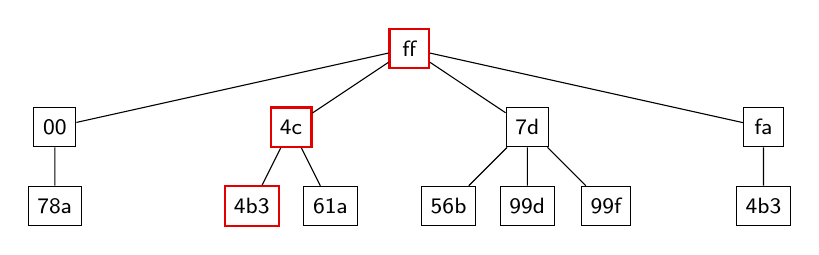
\begin{tikzpicture}[
          every node/.style={font=\sffamily\footnotesize, draw, rectangle, minimum size=5mm, align=center},
          level 1/.style={sibling distance=30mm, level distance=10mm},
          level 2/.style={sibling distance=10mm, level distance=10mm},
          red/.style={draw=red!90!black, thick},
          -, >=stealth
        ]

        \node[red] (root1) {ff}
            child {node {00}
              child {node {78a}}
            }
            child {node[red] {4c}
              child {node[red] {4b3}}
              child {node {61a}}
            }
            child {node {7d}
              child {node {56b}}
              child {node {99d}}
              child {node {99f}}
            }
            child {node {fa}
              child {node {4b3}}
            };
        \end{tikzpicture}
        \end{figure}
    }
\end{frame}

\begin{frame}{Directory trees as Merkle forest}

\begin{figure}
\begin{tikzpicture}[
  every node/.style={font=\sffamily\footnotesize, draw, rectangle, minimum size=5mm, align=center},
  greenborder/.style={draw=green!90!black, thick},
  greenborder2/.style={draw=green!50!black, thick},
  blueborder/.style={draw=cyan!90!black, thick},
  blueborder2/.style={draw=cyan!50!black, thick},
  yellowborder/.style={draw=orange!90!black, thick},
  yellowborder2/.style={draw=orange!50!black, thick},
  level 1/.style={sibling distance=27mm, level distance=5mm},
  level 2/.style={sibling distance=17mm, level distance=7mm},
  level 3/.style={sibling distance=12mm, level distance=7mm},
  -, >=stealth
]

\node (root1) {Agent 1}
  child {node[greenborder] {fe}
    child {node[greenborder2] {fe/2d}
      child {node {0f8.1}}
    }
  }
  child {node[greenborder] {ff}
    child {node[greenborder2] {ff/4c}
      child {node {4b3.1}}
      child {node {61a.1}}
    }
    child {node[greenborder2] {ff/6d}
      child {node {db7.1}}
    }
  };

\node[right=4cm of root1] (root2) {Agent 2}
  child {node[blueborder] {fe}
    child {node[blueborder2] {fe/2d}
      child {node {0f8.2}}
    }
  }
  child {node[blueborder] {ff}
    child {node[blueborder2] {ff/4c}
      child {node {4b3.2}}
      child {node {61a.2}}
    }
    child {node[blueborder2] {ff/6d}
      child {node {db7.2}}
    }
  };

\node (root3) at ($(root1) + (2.5cm,-3cm)$) {Agent 3}
  child {node[yellowborder] {fe}
    child {node[yellowborder2] {fe/2d}
      child {node {0f8.3}}
    }
  }
  child {node[yellowborder] {ff}
    child {node[yellowborder2] {ff/4c}
      child {node {4b3.3}}
      child {node {61a.3}}
    }
    child {node[yellowborder2] {ff/6d}
      child {node {db7.3}}
    }
  };

\end{tikzpicture}
\end{figure}

Each agent sends the Merkle root hashes of their top- and second-level folders to the agent leader.

\end{frame}

\begin{frame}{Aggregated roots}


\begin{figure}[H]
\centering
\begin{tikzpicture}[
  every node/.style={font=\sffamily\footnotesize, draw, rectangle, minimum size=5mm, align=center},
  hash1/.style={draw=green!90!black, thick},
  hash2/.style={draw=cyan!90!black, thick},
  hash3/.style={draw=orange!90!black, thick},
  level distance=8mm,
  sibling distance=15mm,
  <-, >=stealth
]

\node (fe) {\texttt{fe}}
  child {node[hash1] {\texttt{fe}--1}}
  child {node[hash2] {\texttt{fe}--2}}
  child {node[hash3] {\texttt{fe}--3}};

\node[right=4cm of fe] (ff) {\texttt{ff}}
  child {node[hash1] {\texttt{ff}--1}}
  child {node[hash2] {\texttt{ff}--2}}
  child {node[hash3] {\texttt{ff}--3}};

\node[below=2cm of fe](fe/2d) {\texttt{fe/2d}}
  child {node[hash1] {\texttt{fe/2d}--1}}
  child {node[hash2] {\texttt{fe/2d}--2}}
  child {node[hash3] {\texttt{fe/2d}--3}};

\node[right=4cm of fe/2d] (ff/4c) {\texttt{ff/4c}}
  child {node[hash1] {\texttt{ff/4c}--1}}
  child {node[hash2] {\texttt{ff/4c}--2}}
  child {node[hash3] {\texttt{ff/4c}--3}};

\end{tikzpicture}
\end{figure}

The leader builds Merkle trees for each folder, with the agents' Merkle
    root hashes as leaves.


\end{frame}


\begin{frame}[fragile]{Map of hashes}
\footnotesize
\begin{lstlisting}[language=Python, basicstyle=\ttfamily\footnotesize,
                   keywordstyle=\color{blue},
                   commentstyle=\color{gray},
                   stringstyle=\color{teal},
                   showstringspaces=false]
roots = {
    "fe":   "new root hash of fe",
    "ff":   "new root hash of ff",
    "ff/4c":"new root hash of ff/4c",
    # ...
}

agent_roots = {
    "fe": [
        "Agent 1 root hash of fe",
        "Agent 2 root hash of fe",
        "Agent 3 root hash of fe"
    ],
    # ...
    "ff/4c": [
        "Agent 1 root hash of ff/4c",
        "Agent 2 root hash of ff/4c",
        "Agent 3 root hash of ff/4c"
    ],
}
\end{lstlisting}
\end{frame}

\begin{frame}{Map of hashes}

This map allows us to:
\begin{itemize}
    \item Use \texttt{agent\_roots[<some\_folder>][i-th-agent]} when
        the i-th agent is offline.
    \item If an agent is offline during the upload, the
        \texttt{roots[<some\_folder>]} value is still computed using the
        current status of every agent.
\end{itemize}

\end{frame}

\begin{frame}{Check corruptions}

\begin{figure}
\centering
\begin{tikzpicture}[scale=0.6, every node/.style={scale=0.8}]
\begin{umlseqdiag}

    % Define participants
    \umlobject[no ddots, x=0]{Agent 1}
    \umlobject[no ddots, x=9, fill=gray!20, draw=gray]{Agent 2}
    \umlobject[no ddots, x=14]{Agent 3}

    \begin{umlcall}[op=(1a) Get root hash for \texttt{ff}, dt=10, return=Root hash for \texttt{ff}]{Agent 1}{Agent 1}
    \end{umlcall}

    \begin{umlcall}[op=(1b) Get root hash for Agent 2's \texttt{ff}, dt=10, return=\texttt{agent\_roots["ff"][2]}]{Agent 1}{Agent 1}
    \end{umlcall}

    \begin{umlcall}[op=(1c) Get root hash for \texttt{ff}, dt=10, return=Root hash for \texttt{ff}]{Agent 1}{Agent 3}
    \end{umlcall}

    \begin{umlcall}[op=(2a) Raft log with corruption status for \texttt{ff},
        fill=gray!10, dt=10]{Agent 1}{Agent 2}
    \end{umlcall}
    \begin{umlcall}[op=(2b) Raft log with corruption status for \texttt{ff}, fill=red, dt=10]{Agent 1}{Agent 3}
    \end{umlcall}
\end{umlseqdiag}
\end{tikzpicture}
\end{figure}

\end{frame}
